%  LaTeX support: latex@mdpi.com 
%  For support, please attach all files needed for compiling as well as the log file, and specify your operating system, LaTeX version, and LaTeX editor.

%=================================================================
\documentclass[journal,article,submit,pdftex,moreauthors]{Definitions/mdpi} 
% For posting an early version of this manuscript as a preprint, you may use "preprints" as the journal and change "submit" to "accept". The document class line would be, e.g., \documentclass[preprints,article,accept,moreauthors,pdftex]{mdpi}. This is especially recommended for submission to arXiv, where line numbers should be removed before posting. For preprints.org, the editorial staff will make this change immediately prior to posting.

%--------------------
% Class Options:
%--------------------
%----------
% journal
%----------
% Choose between the following MDPI journals:
% civileng, climate, coasts, earth, ecologies, environments,  forests, infrastructures, plants, preprints, remotesensing,  water

%---------
% article
%---------
% The default type of manuscript is "article", but can be replaced by: 
% supfile = supplementary materials

%----------
% submit
%----------
% The class option "submit" will be changed to "accept" by the Editorial Office when the paper is accepted. This will only make changes to the frontpage (e.g., the logo of the journal will get visible), the headings, and the copyright information. Also, line numbering will be removed. Journal info and pagination for accepted papers will also be assigned by the Editorial Office.

%------------------
% moreauthors
%------------------
% If there is only one author the class option oneauthor should be used. Otherwise use the class option moreauthors.

%---------
% pdftex
%---------
% The option pdftex is for use with pdfLaTeX. If eps figures are used, remove the option pdftex and use LaTeX and dvi2pdf.

%=================================================================
% MDPI internal commands
\firstpage{1} 
\makeatletter 
\setcounter{page}{\@firstpage} 
\makeatother
\pubvolume{1}
\issuenum{1}
\articlenumber{0}
\pubyear{2022}
\copyrightyear{2022}
%\externaleditor{Academic Editor: Firstname Lastname}
\datereceived{} 
%\daterevised{} % Only for the journal Acoustics
\dateaccepted{} 
\datepublished{} 
%\datecorrected{} % Corrected papers include a "Corrected: XXX" date in the original paper.
%\dateretracted{} % Corrected papers include a "Retracted: XXX" date in the original paper.
\hreflink{https://doi.org/} % If needed use \linebreak
%\doinum{}
%------------------------------------------------------------------
% The following line should be uncommented if the LaTeX file is uploaded to arXiv.org
%\pdfoutput=1

%=================================================================
% Add packages and commands here. The following packages are loaded in our class file: fontenc, inputenc, calc, indentfirst, fancyhdr, graphicx, epstopdf, lastpage, ifthen, lineno, float, amsmath, setspace, enumitem, mathpazo, booktabs, titlesec, etoolbox, tabto, xcolor, soul, multirow, microtype, tikz, totcount, changepage, attrib, upgreek, cleveref, amsthm, hyphenat, natbib, hyperref, footmisc, url, geometry, newfloat, caption

%=================================================================
%% Please use the following mathematics environments: Theorem, Lemma, Corollary, Proposition, Characterization, Property, Problem, Example, ExamplesandDefinitions, Hypothesis, Remark, Definition, Notation, Assumption
%% For proofs, please use the proof environment (the amsthm package is loaded by the MDPI class).

%=================================================================
% Full title of the paper (Capitalized)
\Title{Remote Sensing Analysis of Resilience and Cover Change in the Grand-Pierre Bay Mangrove Forest, Artibonite, Haiti}

% MDPI internal command: Title for citation in the left column
\TitleCitation{Title}

% Author Orchid ID: enter ID or remove command
\newcommand{\orcidauthorA}{0000-0000-0000-000X} % Add \orcidA{} behind the author's name
%\newcommand{\orcidauthorB}{0000-0000-0000-000X} % Add \orcidB{} behind the author's name

% Authors, for the paper (add full first names)
\Author{Alexandre Erich Sébastien Georges $^{1,\dagger,\ddagger}$\orcidA{}, Mark T. Stacey $^{1,}$ and Firstname Lastname $^{2,\ddagger}$*}

%\longauthorlist{yes}

% MDPI internal command: Authors, for metadata in PDF
\AuthorNames{Firstname Lastname, Firstname Lastname and Firstname Lastname}

% MDPI internal command: Authors, for citation in the left column
\AuthorCitation{Lastname, F.; Lastname, F.; Lastname, F.}
% If this is a Chicago style journal: Lastname, Firstname, Firstname Lastname, and Firstname Lastname.

% Affiliations / Addresses (Add [1] after \address if there is only one affiliation.)
\address[1]{%
$^{1}$ \quad Department of Civil and Environmental Engineering; University of California, Berkeley; Berkeley, CA, USA; aao@ce.berkeley.edu\\
}

% Contact information of the corresponding author
\corres{Correspondence: alexandre\_georges@berkeley.edu; Tel.: +16315900387 (A.E.S.G)}

% Current address and/or shared authorship
\firstnote{Current address: 2126 California St, Apt 6, Berkeley, CA, USA} 
\secondnote{These authors contributed equally to this work.}
% The commands \thirdnote{} till \eighthnote{} are available for further notes

%\simplesumm{} % Simple summary

%\conference{} % An extended version of a conference paper

% Abstract (Do not insert blank lines, i.e. \\) 
\abstract{The Grand-Pierre Bay, south of Gonaives, Haiti hosts the largest mangrove coverage of the country. It is also unique in the Caribbean region because it is the largest river-fed mangrove forest in the Caribbean islands. As such, it is host to extensive biodiversity and is an important socio-economic resource for the Artibonite region in Haiti. However, it has been a victim of anthropogenic pressure, threatening the biodiversity of the forest and its health and extent. This remote sensing analysis will look at how the density and health of the forest have been evolving for the past decade using satellite images from Landsat and PlanetLabs. Using these Machine Learning classification methods and indices, the mangrove cover and health change will be quantified. A second moment of area metric will be used to represent the extent change in the forests and compared to gross cover loss. Using these methods, we have found that the mangrove forest is retreating from its' coastal front while becoming denser inland. This could point to a mechanistic response of mangrove forests to sea-level rise in this region, which patterns will be important to study further in hydrodynamic studies.}

% Keywords
\keyword{mangroves; remote sensing; coasts; Caribbean; Haiti} 

% The fields PACS, MSC, and JEL may be left empty or commented out if not applicable
%\PACS{J0101}
%\MSC{}
%\JEL{}

%%%%%%%%%%%%%%%%%%%%%%%%%%%%%%%%%%%%%%%%%%
% Only for the journal Applied Sciences
%\featuredapplication{Authors are encouraged to provide a concise description of the specific application or a potential application of the work. This section is not mandatory.}
%%%%%%%%%%%%%%%%%%%%%%%%%%%%%%%%%%%%%%%%%%

%%%%%%%%%%%%%%%%%%%%%%%%%%%%%%%%%%%%%%%%%%
% Only for the journal Data
%\dataset{DOI number or link to the deposited data set if the data set is published separately. If the data set shall be published as a supplement to this paper, this field will be filled by the journal editors. In this case, please submit the data set as a supplement.}
%\datasetlicense{License under which the data set is made available (CC0, CC-BY, CC-BY-SA, CC-BY-NC, etc.)}

\begin{document}

\section{Introduction}

The introduction should briefly place the study in a broad context and highlight why it is important. It should define the purpose of the work and its significance. The current state of the research field should be reviewed carefully and key publications cited. Please highlight controversial and diverging hypotheses when necessary. Finally, briefly mention the main aim of the work and highlight the principal conclusions. As far as possible, please keep the introduction comprehensible to scientists outside your particular field of research. Citing a journal paper \cite{ref-journal}. Now citing a book reference \cite{ref-book1,ref-book2} or other reference types \cite{ref-unpublish,ref-communication,ref-proceeding}. Please use the command \citep{ref-thesis,ref-url} for the following MDPI journals, which use author--date citation: Administrative Sciences, Arts, Econometrics, Economies, Genealogy, Humanities, IJFS, Journal of Intelligence, Journalism and Media, JRFM, Languages, Laws, Religions, Risks, Social Sciences, Literature.

\subsection{Study Site}
The Grand-Pierre Bay Mangrove Forest is situated at the estuary of the l’Estere, Artibonite, and La Quinte rivers. It is the largest mangrove cover in Haiti and features a sea -> mangrove -> marsh -> land system.
\subsection{Ongoing Conservation Efforts}
Discuss ongoing conservation efforts here. Might need to interview Mr. Jean Wiener again.
%%%%%%%%%%%%%%%%%%%%%%%%%%%%%%%%%%%%%%%%%%
\section{Materials and Methods}
This analysis makes use of an array of satellite imagery solutions, indices and image classification methods to detect and quantify mangrove cover change during the period extending from 2010 to 2022. The different datasets, data acquisition, classification and analysis methods are as follow:

\subsection{Datasets}
\subsubsection{Landsat}
Landsat 7 and 8 were used to track NDVI changes between the past decade in the region (2010 – 2022). While the resolutions of Landsat 7-8 instruments are lower than other commercially available satellites, it is very convenient for getting numerous readings for long periods of time for a large region. As such, it was mainly used to form time-series of NDVI in the whole forest and certain key regions.

\subsubsection{PlanetLabs}
PlanetLabs data present much higher resolution (3-5m) but fewer bands for analysis. It is also costly to pull near-weekly data from PlanetLabs. As such, observations around the first 2 months of the year, every 3 years, are taken between 2010 and 2022. This data has been used to monitor mangrove cover and coastline change.

\subsection{Workflow}
** Add figure showing workflow **

Low Tides -> Image Acquisition -> NDWI masking -> Kmeans Clustering -> Gross Cover Change -> Polar Moment of Area Metric -> NDVI Timeseries -> dNDVI Analysis

\subsection{Low-Tide Data Acquisition}
The partially submerged nature of mangrove forests can lead to inconsistencies when trying to track their cover using remote sensing, as submerged regions during flood tides can get hidden away from the satellite view depending on the time of observation. As such, it was decided to only get PlanetLabs observations at the lowest tides of the year to observe the maximum cover of the mangrove forests.
To get the tidal schedule at our site, we established a 1:1 relationship between it and the tidal schedule at Port-au-Prince, Haiti, located in the same basin of the La Gonave Gulf. This is accomplished via hydrodynamic modeling in Delft3D-Flow, where measurements of the tidal regime in Port-au-Prince are related to the boundary conditions of the basin by regression. ** Make workflow plot explaining this process better **. 
With the tidal regime at our site in hand, we can then select available satellite imagery at the lowest available tidal ranges every year. 

\subsection{Image Classification}
\subsubsection{K-means Clustering}
"k-means clustering is a method of vector quantization, originally from signal processing, that aims to partition n observations into k clusters in which each observation belongs to the cluster with the nearest mean (cluster centers or cluster centroid), serving as a prototype of the cluster. This results in a partitioning of the data space into Voronoi cells. k-means clustering minimizes within-cluster variances (squared Euclidean distances), but not regular Euclidean distances, which would be the more difficult Weber problem: the mean optimizes squared errors, whereas only the geometric median minimizes Euclidean distances. For instance, better Euclidean solutions can be found using k-medians and k-medoids."

We use K-means clustering on the surface reflectance values to classify the different land cover into 4 types: open water, mangrove vegetation, bare soil 1 (bare sand), and bare soil 2 (mud flat). After masking out the open water and bare soil covers, the remaining mangrove vegetation covers are compared over years to track the patterns in mangrove cover change.

\subsubsection{Deep Learning Classification}
??? (Potential Future Work.)
\subsubsection{Gross Cover Loss and Second Moment of Area}
Using the final mangrove cover extents, we calculate two metrics to quantify and characterize the cover change patterns in subregions: gross cover loss and polar moment of area.
With Gross Cover Loss (GCL), we simply take the difference in covered pixels between 2022 and 2010, multiplying that number of pixels by the unit pixel area to obtain an area in km sq. 

The polar moment of area (MOA) on the other looks at the distribution of those pixels related to the center of the extent of a subregion. The second moment of area (2MOA) of the mangrove cover is calculated in relation to the center x and y axes as a sum of the 2MOAs of all pixels:

\[I_x = \sum{A\times d_x^2} \] 
\[I_y = \sum{A\times d_y^2} \]

The overall MOA metric is then the sum of $I_{x}$ and $I_{y}$:
\[MOA (J_z) = I_x + I_z \]

\subsection{Indices}
\subsubsection{NDWI Masking Pre-Processing}
To simplify the clustering process of, we mask out the open water regions surrounding the mangrove forest. This is done using the green and NIR bands of PlanetLabs, following the relation defined by McFeeters (1996):
\[NDWI = \frac {Xgreen - Xnir}{Xgreen + Xnir} \]
The resulting masked out images are then used in our classifications and analyses.

\subsubsection{NDVI Analysis}
The land surfaces that we find after masking out open water using NDWI are analyzed by NDVI to gauge the change in health of the forest. NDVI (Normalized Difference Vegetation Index) is a simple indicator of the presence, density and health of green vegetation. This index uses the green and near-infrared bands of observations as follow:
\[NDVI = \frac{Xnir - Xred}{Xnir + Xred}\]
To gauge the change in health, we look at the spatial difference of the NDVI distribution between 2022 and 2010:
\[dNDVI = NDVI_{2022} - NDVI_{2010}\]
Additionally, the average NDVI of Landsat observations over that time period are used for time-series showing trends of NDVI change in more detail.
%%%%%%%%%%%%%%%%%%%%%%%%%%%%%%%%%%%%%%%%%%
\section{Results}
\subsection{Mangrove Detection and Cover Change Metrics}
**Cover change visualizations here**
**GCL and MOA tables and figures here**

\begin{figure}[H]
\includegraphics[width=13.5 cm]{Figures/visualisation_water_mask.png}
\caption{Visualization of areas of interest with open water masked. The mangrove forest was divided in 7 subregions from a 3x3 grid which were named according to their cardinal directions.\label{fig1}}
\end{figure}  

\begin{figure}[H]
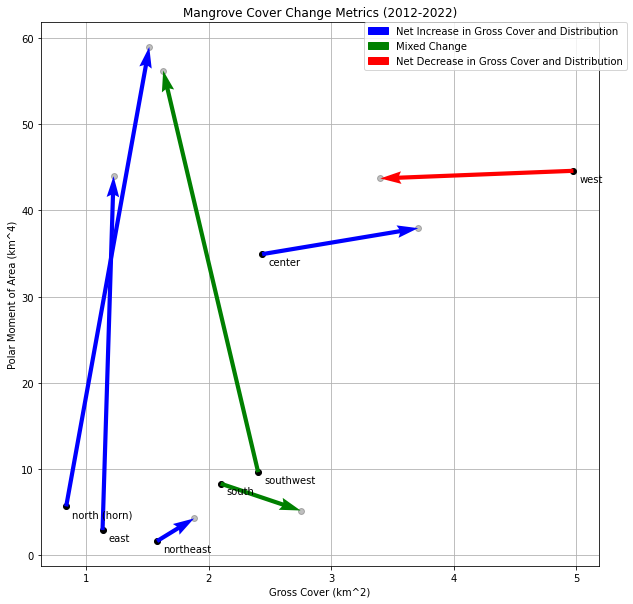
\includegraphics[width=13.5 cm]{Figures/mangrove_change_metric.png}
\caption{Metrics displaying the change patterns in the mangrove cover in the different subregions. \label{fig2}}
\end{figure}  

\subsection{dNDVI Analysis}
**dNDVI figures here**
\begin{figure}[H]
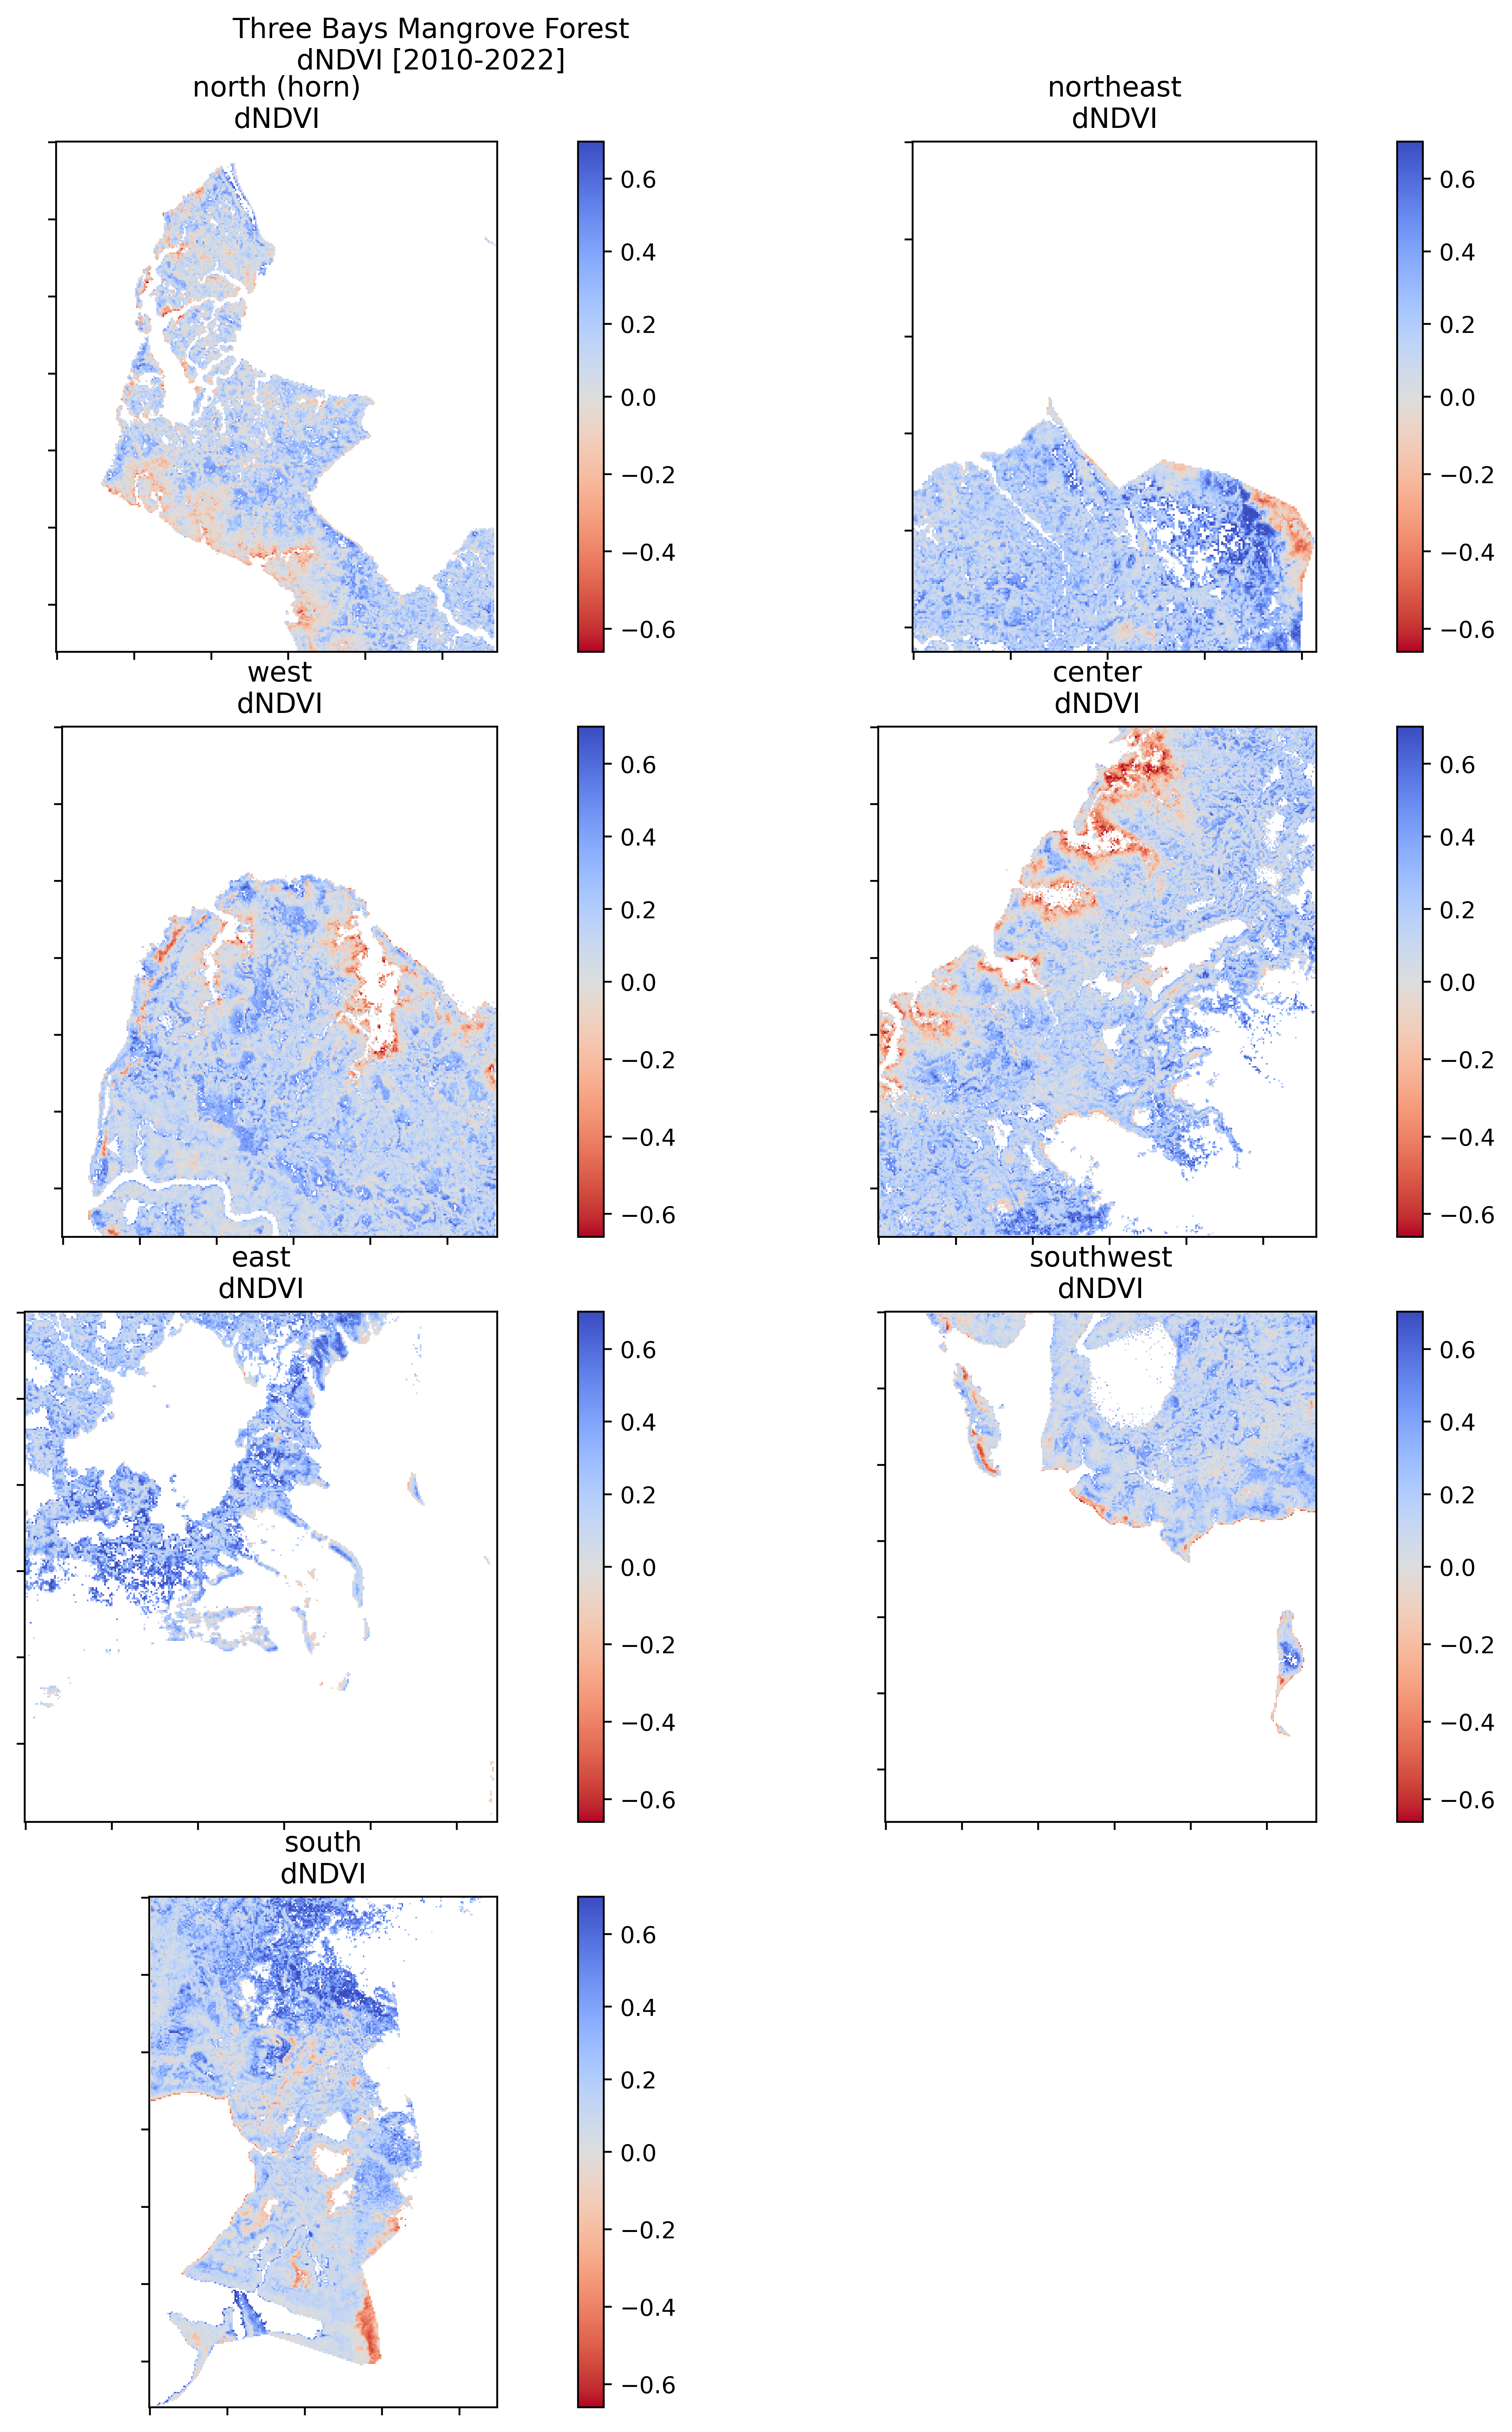
\includegraphics[width=13.5 cm]{Figures/mangrove_ndvi.png}
\caption{dNDVI graphical analysis of the different subregions between 2022 and 2010. \label{fig3}}
\end{figure}  

\subsection{NDVI Timeseries Analysis}
**NDVI timeseries here**
Timeseries of the mean and maximum NDVI in the Grand-Pierre Bay have been taken. Areas of interest were the mangrove forest, the Gulf of Gonave coast of the forest, and the “brackish Grand Pierre” lake coast. 


The text continues here. 



All figures and tables should be cited in the main text as Figure~\ref{fig1}, Table~\ref{tab1}, Table~\ref{tab2}, etc.

 
\unskip

\begin{table}[H] 
\caption{Gross Cover Change in Forest Subregions\label{tab1}}
\newcolumntype{C}{>{\centering\arraybackslash}X}
\begin{tabularx}{\textwidth}{CCC}
\toprule
\textbf{AOI}	& \textbf{Gross Cover Change}	& \textbf{Gross Percent Change}\\
\midrule
North (Horn)		& 0.678195			& 81.123\\
Northeast		& 0.302			& 19.132\\
West            & -1.577        & -31.681\\
Center          & 1.274         & 52.298\\
East            & 0.0899        & 7.936\\
Southwest       & -0.775        & -32.265\\
South           & 0.652         & 31.094\\
\bottomrule
\end{tabularx}
\end{table}
\unskip

\begin{table}[H]
\caption{This is a wide table.\label{tab2}}
	\begin{adjustwidth}{-\extralength}{0cm}
		\newcolumntype{C}{>{\centering\arraybackslash}X}
		\begin{tabularx}{\fulllength}{CCCCC}
			\toprule
			\textbf{AOI}	& \textbf{Gross Cover Change}	& \textbf{Gross Percent Change}     & \textbf{Polar 2MOA Change}      &\textbf{Polar 2MOA Percent Change}\\
			\midrule
North (Horn)		& 0.678195			& 81.123    & 53.295    & 941.644\\
Northeast		& 0.302			& 19.132    & 2.631     & 1260.764\\
West            & -1.577        & -31.681   & -0.887    & -1.989\\
Center          & 1.274         & 52.298    & 3.016     & 8.638\\
East            & 0.0899        & 7.936     & 41.043    & 1408.445\\
Southwest       & -0.775        & -32.265   & 46.579    & 483.698\\
South           & 0.652         & 31.094    & -3.114    & -37.524\\
			\bottomrule
		\end{tabularx}
	\end{adjustwidth}
	\noindent{\footnotesize{\textsuperscript{1} This is a table footnote.}}
\end{table}

%\begin{listing}[H]
%\caption{Title of the listing}
%\rule{\columnwidth}{1pt}
%\raggedright Text of the listing. In font size footnotesize, small, or normalsize. Preferred format: left aligned and single spaced. Preferred border format: top border line and bottom border line.
%\rule{\columnwidth}{1pt}
%\end{listing}

Text.

Text.

\subsection{Formatting of Mathematical Components}

This is the example 1 of equation:
\begin{linenomath}
\begin{equation}
a = 1,
\end{equation}
\end{linenomath}
the text following an equation need not be a new paragraph. Please punctuate equations as regular text.
%% If the documentclass option "submit" is chosen, please insert a blank line before and after any math environment (equation and eqnarray environments). This ensures correct linenumbering. The blank line should be removed when the documentclass option is changed to "accept" because the text following an equation should not be a new paragraph.

This is the example 2 of equation:
\begin{adjustwidth}{-\extralength}{0cm}
\begin{equation}
a = b + c + d + e + f + g + h + i + j + k + l + m + n + o + p + q + r + s + t + u + v + w + x + y + z
\end{equation}
\end{adjustwidth}

% Example of a page in landscape format (with table and table footnote).
%\startlandscape
%\begin{table}[H] %% Table in wide page
%\caption{This is a very wide table.\label{tab3}}
%	\begin{tabularx}{\textwidth}{CCCC}
%		\toprule
%		\textbf{Title 1}	& \textbf{Title 2}	& \textbf{Title 3}	& \textbf{Title 4}\\
%		\midrule
%		Entry 1		& Data			& Data			& This cell has some longer content that runs over two lines.\\
%		Entry 2		& Data			& Data			& Data\textsuperscript{1}\\
%		\bottomrule
%	\end{tabularx}
%	\begin{adjustwidth}{+\extralength}{0cm}
%		\noindent\footnotesize{\textsuperscript{1} This is a table footnote.}
%	\end{adjustwidth}
%\end{table}
%\finishlandscape

% Example of a figure that spans the whole page width. The same concept works for tables, too.
\begin{figure}[H]
\begin{adjustwidth}{-\extralength}{0cm}
\centering
\includegraphics[width=13.5cm]{Figures/mangrove_masked.png}
\end{adjustwidth}
\caption{Masked mangrove covers from observations.\label{fig2}}
\end{figure}  

Please punctuate equations as regular text. Theorem-type environments (including propositions, lemmas, corollaries etc.) can be formatted as follows:
%% Example of a theorem:
\begin{Theorem}
Example text of a theorem.
\end{Theorem}

The text continues here. Proofs must be formatted as follows:

%% Example of a proof:
\begin{proof}[Proof of Theorem 1]
Text of the proof. Note that the phrase ``of Theorem 1'' is optional if it is clear which theorem is being referred to.
\end{proof}
The text continues here.

%%%%%%%%%%%%%%%%%%%%%%%%%%%%%%%%%%%%%%%%%%
\section{Discussion}

Authors should discuss the results and how they can be interpreted from the perspective of previous studies and of the working hypotheses. The findings and their implications should be discussed in the broadest context possible. Future research directions may also be highlighted.

%%%%%%%%%%%%%%%%%%%%%%%%%%%%%%%%%%%%%%%%%%
\section{Conclusions}

This section is not mandatory, but can be added to the manuscript if the discussion is unusually long or complex.

%%%%%%%%%%%%%%%%%%%%%%%%%%%%%%%%%%%%%%%%%%
\section{Patents}

This section is not mandatory, but may be added if there are patents resulting from the work reported in this manuscript.

%%%%%%%%%%%%%%%%%%%%%%%%%%%%%%%%%%%%%%%%%%
\vspace{6pt} 

%%%%%%%%%%%%%%%%%%%%%%%%%%%%%%%%%%%%%%%%%%
%% optional
%\supplementary{The following supporting information can be downloaded at:  \linksupplementary{s1}, Figure S1: title; Table S1: title; Video S1: title.}

% Only for the journal Methods and Protocols:
% If you wish to submit a video article, please do so with any other supplementary material.
% \supplementary{The following supporting information can be downloaded at: \linksupplementary{s1}, Figure S1: title; Table S1: title; Video S1: title. A supporting video article is available at doi: link.}

%%%%%%%%%%%%%%%%%%%%%%%%%%%%%%%%%%%%%%%%%%
\authorcontributions{For research articles with several authors, a short paragraph specifying their individual contributions must be provided. The following statements should be used ``Conceptualization, X.X. and Y.Y.; methodology, X.X.; software, X.X.; validation, X.X., Y.Y. and Z.Z.; formal analysis, X.X.; investigation, X.X.; resources, X.X.; data curation, X.X.; writing---original draft preparation, X.X.; writing---review and editing, X.X.; visualization, X.X.; supervision, X.X.; project administration, X.X.; funding acquisition, Y.Y. All authors have read and agreed to the published version of the manuscript.'', please turn to the  \href{http://img.mdpi.org/data/contributor-role-instruction.pdf}{CRediT taxonomy} for the term explanation. Authorship must be limited to those who have contributed substantially to the work~reported.}

\funding{Please add: ``This research received no external funding'' or ``This research was funded by NAME OF FUNDER grant number XXX.'' and  and ``The APC was funded by XXX''. Check carefully that the details given are accurate and use the standard spelling of funding agency names at \url{https://search.crossref.org/funding}, any errors may affect your future funding.}

\institutionalreview{In this section, you should add the Institutional Review Board Statement and approval number, if relevant to your study. You might choose to exclude this statement if the study did not require ethical approval. Please note that the Editorial Office might ask you for further information. Please add “The study was conducted in accordance with the Declaration of Helsinki, and approved by the Institutional Review Board (or Ethics Committee) of NAME OF INSTITUTE (protocol code XXX and date of approval).” for studies involving humans. OR “The animal study protocol was approved by the Institutional Review Board (or Ethics Committee) of NAME OF INSTITUTE (protocol code XXX and date of approval).” for studies involving animals. OR “Ethical review and approval were waived for this study due to REASON (please provide a detailed justification).” OR “Not applicable” for studies not involving humans or animals.}

\informedconsent{Any research article describing a study involving humans should contain this statement. Please add ``Informed consent was obtained from all subjects involved in the study.'' OR ``Patient consent was waived due to REASON (please provide a detailed justification).'' OR ``Not applicable'' for studies not involving humans. You might also choose to exclude this statement if the study did not involve humans.

Written informed consent for publication must be obtained from participating patients who can be identified (including by the patients themselves). Please state ``Written informed consent has been obtained from the patient(s) to publish this paper'' if applicable.}

\dataavailability{In this section, please provide details regarding where data supporting reported results can be found, including links to publicly archived datasets analyzed or generated during the study. Please refer to suggested Data Availability Statements in section ``MDPI Research Data Policies'' at \url{https://www.mdpi.com/ethics}. If the study did not report any data, you might add ``Not applicable'' here.} 

\acknowledgments{In this section you can acknowledge any support given which is not covered by the author contribution or funding sections. This may include administrative and technical support, or donations in kind (e.g., materials used for experiments).}

\conflictsofinterest{Declare conflicts of interest or state ``The authors declare no conflict of interest.'' Authors must identify and declare any personal circumstances or interest that may be perceived as inappropriately influencing the representation or interpretation of reported research results. Any role of the funders in the design of the study; in the collection, analyses or interpretation of data; in the writing of the manuscript; or in the decision to publish the results must be declared in this section. If there is no role, please state ``The funders had no role in the design of the study; in the collection, analyses, or interpretation of data; in the writing of the manuscript; or in the decision to publish the~results''.} 

%%%%%%%%%%%%%%%%%%%%%%%%%%%%%%%%%%%%%%%%%%
%% Optional
\sampleavailability{Samples of the compounds ... are available from the authors.}

%% Only for journal Encyclopedia
%\entrylink{The Link to this entry published on the encyclopedia platform.}

\abbreviations{Abbreviations}{
The following abbreviations are used in this manuscript:\\

\noindent 
\begin{tabular}{@{}ll}
MDPI & Multidisciplinary Digital Publishing Institute\\
DOAJ & Directory of open access journals\\
TLA & Three letter acronym\\
LD & Linear dichroism
\end{tabular}
}

%%%%%%%%%%%%%%%%%%%%%%%%%%%%%%%%%%%%%%%%%%
%% Optional
\appendixtitles{no} % Leave argument "no" if all appendix headings stay EMPTY (then no dot is printed after "Appendix A"). If the appendix sections contain a heading then change the argument to "yes".
\appendixstart
\appendix
\section[\appendixname~\thesection]{}
\subsection[\appendixname~\thesubsection]{}
The appendix is an optional section that can contain details and data supplemental to the main text---for example, explanations of experimental details that would disrupt the flow of the main text but nonetheless remain crucial to understanding and reproducing the research shown; figures of replicates for experiments of which representative data are shown in the main text can be added here if brief, or as Supplementary Data. Mathematical proofs of results not central to the paper can be added as an appendix.

\begin{table}[H] 
\caption{This is a table caption.\label{tab5}}
\newcolumntype{C}{>{\centering\arraybackslash}X}
\begin{tabularx}{\textwidth}{CCC}
\toprule
\textbf{Title 1}	& \textbf{Title 2}	& \textbf{Title 3}\\
\midrule
Entry 1		& Data			& Data\\
Entry 2		& Data			& Data\\
\bottomrule
\end{tabularx}
\end{table}

\section[\appendixname~\thesection]{}
All appendix sections must be cited in the main text. In the appendices, Figures, Tables, etc. should be labeled, starting with ``A''---e.g., Figure A1, Figure A2, etc.

%%%%%%%%%%%%%%%%%%%%%%%%%%%%%%%%%%%%%%%%%%
\begin{adjustwidth}{-\extralength}{0cm}
%\printendnotes[custom] % Un-comment to print a list of endnotes

\reftitle{References}

% Please provide either the correct journal abbreviation (e.g. according to the “List of Title Word Abbreviations” http://www.issn.org/services/online-services/access-to-the-ltwa/) or the full name of the journal.
% Citations and References in Supplementary files are permitted provided that they also appear in the reference list here. 

%=====================================
% References, variant A: external bibliography
%=====================================
%\bibliography{your_external_BibTeX_file}

%=====================================
% References, variant B: internal bibliography
%=====================================
\begin{thebibliography}{999}
% Reference 1
\bibitem[Author1(year)]{ref-journal}
Author~1, T. The title of the cited article. {\em Journal Abbreviation} {\bf 2008}, {\em 10}, 142--149.
% Reference 2
\bibitem[Author2(year)]{ref-book1}
Author~2, L. The title of the cited contribution. In {\em The Book Title}; Editor 1, F., Editor 2, A., Eds.; Publishing House: City, Country, 2007; pp. 32--58.
% Reference 3
\bibitem[Author3(year)]{ref-book2}
Author 1, A.; Author 2, B. \textit{Book Title}, 3rd ed.; Publisher: Publisher Location, Country, 2008; pp. 154--196.
% Reference 4
\bibitem[Author4(year)]{ref-unpublish}
Author 1, A.B.; Author 2, C. Title of Unpublished Work. \textit{Abbreviated Journal Name} year, \textit{phrase indicating stage of publication (submitted; accepted; in press)}.
% Reference 5
\bibitem[Author5(year)]{ref-communication}
Author 1, A.B. (University, City, State, Country); Author 2, C. (Institute, City, State, Country). Personal communication, 2012.
% Reference 6
\bibitem[Author6(year)]{ref-proceeding}
Author 1, A.B.; Author 2, C.D.; Author 3, E.F. Title of presentation. In Proceedings of the Name of the Conference, Location of Conference, Country, Date of Conference (Day Month Year); Abstract Number (optional), Pagination (optional).
% Reference 7
\bibitem[Author7(year)]{ref-thesis}
Author 1, A.B. Title of Thesis. Level of Thesis, Degree-Granting University, Location of University, Date of Completion.
% Reference 8
\bibitem[Author8(year)]{ref-url}
Title of Site. Available online: URL (accessed on Day Month Year).
\end{thebibliography}

% If authors have biography, please use the format below
%\section*{Short Biography of Authors}
%\bio
%{\raisebox{-0.35cm}{\includegraphics[width=3.5cm,height=5.3cm,clip,keepaspectratio]{Definitions/author1.pdf}}}
%{\textbf{Firstname Lastname} Biography of first author}
%
%\bio
%{\raisebox{-0.35cm}{\includegraphics[width=3.5cm,height=5.3cm,clip,keepaspectratio]{Definitions/author2.jpg}}}
%{\textbf{Firstname Lastname} Biography of second author}

% For the MDPI journals use author-date citation, please follow the formatting guidelines on http://www.mdpi.com/authors/references
% To cite two works by the same author: \citeauthor{ref-journal-1a} (\citeyear{ref-journal-1a}, \citeyear{ref-journal-1b}). This produces: Whittaker (1967, 1975)
% To cite two works by the same author with specific pages: \citeauthor{ref-journal-3a} (\citeyear{ref-journal-3a}, p. 328; \citeyear{ref-journal-3b}, p.475). This produces: Wong (1999, p. 328; 2000, p. 475)

%%%%%%%%%%%%%%%%%%%%%%%%%%%%%%%%%%%%%%%%%%
%% for journal Sci
%\reviewreports{\\
%Reviewer 1 comments and authors’ response\\
%Reviewer 2 comments and authors’ response\\
%Reviewer 3 comments and authors’ response
%}
%%%%%%%%%%%%%%%%%%%%%%%%%%%%%%%%%%%%%%%%%%
\end{adjustwidth}
\end{document}

